\chapter{Rozšíření dynamického rozsahu, potlačování šumu a rušení}
Pro co nejpřesnější měření je nezbytné dosáhnout co největšího SNR (signal to noise ratio). Prvním limitujícím faktorem je dynamický rozsah ADC. V případě měření v reálném čase by bylo možné použít nanejvýš osmibitové převodníky, které mají dynamiku přibližně \SI{48}{\deci\bel} podle vztahu
\begin{equation}
	 DR=20log\left(\frac{2^n-1}{1}\right)
\end{equation}
Pro nižší rychlosti jsou dostupné již ADC s vyšší přesností, někdy již integrované přímo do mikrokontrolérů. Běžně se integrují převodníky až do \SI{1}{\megasample} při rozlišení 12~bitů, tedy s dynamickým rozsahem přibližně
\begin{equation}
	DR=20log\left(\frac{2^{12}-1}{1}\right) \doteq \SI{72}{\deci\bel}
\end{equation}

Pro aplikace ve zvukové technice jsou pak dostupné šestnáctibitové až dvacetičtyřbitové převodníky (obvykle do 96 kSa/s) s dynamikou od 
\begin{equation}
	DR=20log\left(\frac{2^{16}-1}{1}\right) \doteq \SI{96}{\deci\bel}
\end{equation} až do
\begin{equation}
	DR=20log\left(\frac{2^{24}-1}{1}\right) \doteq \SI{144}{\deci\bel}
\end{equation}
 Druhý údaj je však pouze teoretický, převodníky sice nabízejí tento počet bitů, ovšem jejich vlastní šum zpravidla omezuje použitelný rozsah na méně než \SI{100}{\deci\bel}. Přesné \SI{24}{\bit} převodníky, které mají skutečně dynamický rozsah odpovídající počtu bitů, vzorkují zpravidla nanejvýš na desítkách \si{\hertz}. Takové rychlosti jsou však pro použití v reflektometru příliš pomalé, neboť změření odezvy systému by bylo velice zdlouhavé.

Vzhledem k rychlosti se zdají být použitelné nanejvýš \SIrange{12}{16}{bitové} převodníky. Existují ovšem metody rozšíření dynamického rozsahu, zpravidla spoléhající na zkreslení měřených dat nelineární funkcí, která umožní navzorkovaná data inverzní funkcí převést zpět na původní signál, přičemž ale nedojde ke ztrátě přesnosti, nýbrž k jejímu zlepšení v určité části převodní charakteristiky. Pro účely telefonie se v minulosti používaly například komprese definované ve standardu G.711 od ITU-T. Tyto komprese umožňovaly komprimovat logaritmicky enkódovaná data z 14~bitů na 8, přičemž uživatel po dekompresi pozoroval výrazně menší zkreslení, než k jakému by došlo, pokud by bylo použita přímo osmibitová kvantizace.

Pro účely měření vysokofrekvenčních signálů se vyrábí logaritmické detektory s rozsahem až \SI{100}{\deci\bel} \cite{AD8309datasheet} \ref{ad8309function}. Pro nízké frekvence poskytuje např. detektor AD8309 \SI{85}{\deci\bel} dynamického rozsahu při toleranci $\pm \SI{1}{\deci\bel}$. Logaritmus je prostá funkce, je tedy možné spočítat její inverzní funkci. Podle \ref{ad8309function} odpovídá vstupnímu rozsahu \SIrange{-70}{10}{\deci\bel m} výstupní rozsah o velikosti \SI{1.5}{\volt}. Při uvažování převodníku s referencí \SI{3.3}{\volt} a rozlišení 12~bitů odpovídá nejmenší měřitelný rozdíl napětí převodníkem \SI{0.8}{\milli\volt}, což s detektorem odpovídá vstupnímu rozlišení přibližně \SI{0.043}{\deci\bel}. Kombinací takového detektoru s dvanáctibitovým převodníkem a proložením dat získaných z lineárního a logaritmického měření je možné vytvořit převodník, který se přesností blíží rychlému šestnáctibitovému převodníku.

\begin{figure}[htbp]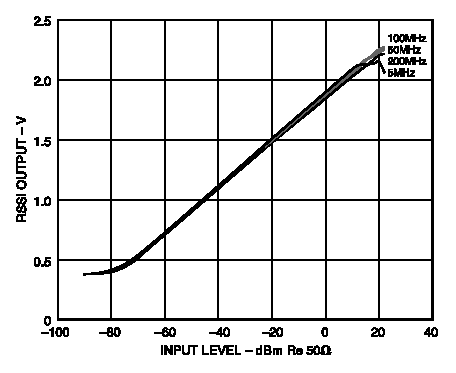
\includegraphics[width=0.8\textwidth,keepaspectratio]{images/AD8309_function.eps}\caption{Převodní funkce logaritmického detektoru AD8309 \cite{AD8309datasheet}}\label{ad8309function}\end{figure}	

\begin{figure}[htbp]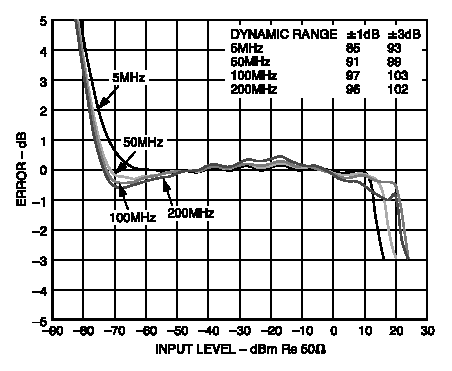
\includegraphics[width=0.8\textwidth,keepaspectratio]{images/AD8309_error.eps}\caption{Chyba převodní funkce logaritmického detektoru AD8309 \cite{AD8309datasheet}}\label{ad8309error}\end{figure}

Pro potlačení šumu v měřeném průběhu je možné použít velké převzorkování signálu a aplikovat na tato data filtr pro potlačení šumu mimo užitečné pásmo. Dále je možné měřený průběh opakovaně měřit a statisticky zpracovávat (buď jednoduchým průměrem nebo např. Kalmanovými filtry).

Použitím měření v ekvivalentním čase je také možné redukovat rušení z okolí za předpokladu, že žádný násobek tohoto rušivého signálu není přesně roven vzorkovacímu kmitočtu. Pak se toto rušení projeví jako šum, který je možné odstranit či alespoň potlačit metodami zmíněnými v předchozím odstavci. V opačném případě je možné rušení potlačit pouze tak, že se provede měření s jinou vzorkovací frekvencí.